\documentclass[12pt]{article}
\usepackage{sd}

\title{Stadium Traffic}
\team{13}
\addauthor{Parth Doshi;parthd@seas.upenn.edu}
\addauthor{Zain Mukaty;zmukaty@seas.upenn.edu}
\addauthor{Felipe Ochoa;felipeo@seas.upenn.edu}
\advisor{Dr. Andrew E. Huemmler;huemmler@seas.upenn.edu}
\reportname{Phase 2 Project Report}
\addbibresource{../sources.bib}

\begin{document}
\maketitle
\abstract

Lincoln Financial Field, the home stadium of the Philadelphia Eagles,
the Philadelphia Union, and the Temple Owls, is located within city
limits and is accessible by car, train and bus. The seven home games
of the Eagles' season this year have drawn an average crowd of
69,144. \cite{espn-attendance} All these fans generate greenhouse
gases traveling to and from the stadium.

Over the past decade, the Eagle's have been making efforts to become
more environmentally friendly, including recycling, conservation,
and sourcing. \cite{eagles-go-green}  They also offer tips for
fans who want to help with this mission. No significant efforts have
been made so far, however, to quantify and reduce the
environmental footprint of these fans traveling to and from the stadium.

This system meets two important needs that would help the Eagles and
their fans further reduce their carbon footprint.

First, it quantifies the average amount of emissions generated in this
manner every time the Eagles have a home game. This calculation is
carried out by a Greenhouse gas calculator based on the average
distance traveled by Eagles fans and on the types of transportation
they use. These parameters are in turn estimated by a comprehensive
traffic model.

Second, the system provides a simulation tool that can estimate how
emissions change in response to shifts in fan behavior, and in turn
how such behavior can change in response to certain incentives. This
tool thus gives Eagles management a way to analyze the potential
impact of an incentive scheme for fans that could complement their Go
Green initiative.

\newpage

\tableofcontents

\newpage

\mainmatter

\section{Introduction}
\subsection{Overview}
Stadium Traffic aims to reduce the greenhouse gas (GHG) emissions from people going
to and from sports games. In particular, our project will focus on the
Philadelphia Eagles and Phillies stadiums.  We aim to build a model
that can be used to quantify the GHG emissions generated due to
people coming to and going from games. We will then develop solutions
to reduce the number of people coming by cars or leave over longer
time period and develop a traffic routing algorithm, aiming to reduce
the GHG emissions from idling cars waiting to leave the stadium. We
will test these on our model to find a successful combination. If we
can get the cooperation of Phillies/Eagles/Flyers and Philadelphia Police
Department, we hope to work with them to implement the results of our
project.

\subsection{Motivation}
All of us have been to large gatherings like
sports games, concerts or conferences and can therefore relate to the
traffic problems when everyone is trying to leave at the same time at
the end of the event. However, what most people don’t realize is the
environmental effect of this traffic. Our project aims to find
solutions to reduce this traffic and hence reduce the emissions while
cars idle in parking lots trying to leave.

The project is focusing on the Philadelphia Eagles, Phillies and Flyers
stadiums. Sports events draw huge crowds at peak traffic
hours and are therefore a great instance on which to model our
project. The Eagles are also undertaking a Go Green! initiative, which
is a push towards becoming more environmentally conscious. Some
initiatives that they have taken are the use of renewable energy
sources for their power consumption and using cups and plates made
from recycled materials. We believe that we can get the support of the
Eagles for our project, as it can be part of the Go Green! initiative
and further reduce the carbon footprint of the stadium.

When the football or baseball game ends, everyone tries to the leave
the stadium at the same time. Although traffic police conduct the
traffic, they do it in a haphazard way. Furthermore, the decision of
which gates to be open and which ones to remain closed is also done
using intuition rather than any efficiency-maximizing algorithm. We
saw this inefficient process as an opportunity to develop an algorithm
to reduce car idling time and GHG emissions.

\subsection{Project Goal and Objectives}
Although the overarching aim of our project is to reduce GHG
emissions due to people going to/from the sports games, we broke this
down into certain specific and measurable objectives:

\begin{enumerate}
    \item Develop a comprehensive model of transportation to and from
  the stadium.
    \item Quantify the total emissions due to transportation to/from
  games.
    \item Develop a tool to simulate the emissions impact of various
  initiatives to reduce private transportation usage (e.g. offering a
  discounted drink to someone who rides the SEPTA).
    \item Create an algorithm to optimally route exiting vehicle traffic
  according to total emissions generated.
    \item Develop a method for the Philadelphia traffic police to
  implement the traffic routing recommendations of our project.
\end{enumerate}

The success of each of the objectives can be measured and how we would
measure the success is stated below:

We would consider a success model one that takes inputs such as trip
distribution, number of attendees, start and end time and produces
outputs such as average idling time and number of cars.

The aim of the project is to reduce GHG emissions, so we need to be
able to measure and quantify GHG emissions from idling cars.

Our model should be able to quantify the effect of different
incentives on GHG emissions so that we can test different
strategies and find the optimal combination.

Optimal routing of traffic can impact GHG emissions from idling
cars, so we need to create an algorithm that can be constraint
optimized. A working algorithm can help the traffic police conduct
traffic in a more organized manner.

Having a front-end system that can be used by the Philadelphia Police
will allow our algorithm to be implemented and hence allow our project
to have an impact. Therefore we need a mock-up of a computer or phone application
that can be used by the police while conducting traffic.

\subsection{Constraints}
The main constraint is the cooperation of the Philadelphia
Eagles/Phillies/Flyers and Philadelphia Police Department because without
their cooperation we cannot implement our project. However, our
advisor Dr. Huemmler has good relationships with both sets of organizations
and has been trying to get their support for the project.

Another constraint is the team’s lack of experience with
transportation engineering.  Since the project involves the
understanding, modeling and optimizing of transport systems, this
would be a constraint. However, we have taken an initiative to get the
help of Professor Vukan Vuchic, a senior professor in transport
engineering, and began familiarizing ourselves with relevant transport
systems concepts under his guidance.

Finally, our last constraint is the data collection required to build
a representative model. However, we have been trying to get the
required information from the Eagles, Phillies, Flyers and other government
departments.

\section{Discussion of Previous Work}
\subsection{Scholarly Work}
Scholarly research in transportation model distinguishes between two
broad approaches: \cite{kitamura1988}

\begin{description}[style=nextline]
    \item[Activity-based] Modeled at the individual level. Considers
  trips arising from different activities that comprise a tour. (E.g.,
  travel to kids' school, then to work, then to the grocery store, and
  finally back home). \cite{kitamura1988}
    \item[Trip-based] Modeled at the Traffic Analysis Zone (TAZ)
  level. Considers broader characteristics such as demographics of a
  neighborhood to model trip times and volumes.\cite{murthy01}
\end{description}

The activity-based model dominates in the most recent academic
literature, but from our survey, the trip-based model still appears to
be the most frequently used type of model by government
agencies. Within the trip-based models the dominant kind appears to be
the four-stage model, which breaks down into four components:
\cite{murthy01}

\begin{enumerate}
    \item Trip Generation
    \item Trip Distribution
    \item Mode Choice
    \item Trip Assignment
\end{enumerate}

In all the applications we've seen, each of those stages is further
refined by the category of the trip being modeled. The usual breakdown
is:

\begin{description}
  \item[Home-based work] (HBW) Trips from home to work or vice versa.
  \item[Home-based shop] (HBS) Trips from home to go shopping and back
(sometimes omitted).
  \item[Home-based other](HBO) Other trips having the home as an
origin or destination.
  \item[Non-home-based work] (NHW) Trips to or from work not in HBWl
  \item[Non-home-based other](NHO) All other kinds of trips.
\end{description}

One of the main benefits of the trip-based approach is its long
history and current widespread use. The model is also readily
modularized, and can be easily adapted and specialized for our
purposes. On the other hand, it is more simplistic than the
activity-based model, since it ignores the interactions of past trips
generated on future trip generation. The activity-based model,
however, has a clear computational disadvantage. The level of detail
the model reaches means that it is very demanding computationally, and
is also hard to break into subcomponents.

Our approach will combine aspects from both styles (as detailed in
section 3), but will borrow the terminology of the trip-based style.

\subsubsection{Phoenix, Arizona Planning Authority}
In 2011 the planning authority in Phoenix, Arizona, MAG, undertook an
extensive project to model transit movement to planned special events
in the region. \cite{kuppam11} Our chosen topic, sports games, falls
under their category of a planned special event. The authors identify
the proportion of special events patrons who utilized light rail
v. alternative modes of transportation and their approach to modeling
demand and modal choice for this event. While the results are specific
to their application, the methodology can be adapted to our specific
focus.

\subsubsection{ITE Trip Generation Database}
The ITE compiled a database with various data patterns related to Trip
Generation. \cite{ite08} We will be able to use the information it contains,
specifically the information related to the special events travel,
e.g. sports games and movies.

\subsubsection{Robertson Stadium}
Gunda Corporation performed a relatively similar project to the one we
are developing for Robertson Stadium at the University of
Houston.\cite{gunda} Although the stadium has a lower capacity than
the Eagles stadium, \cite{robertson-stadium} it is home to an MLS
team, and has to abide by all the traffic management principles of a
professional sports team. The scope and aim of Gunda's analysis
differed from our own, but their analysis can strongly inform a
component of our model. (The micro-car module, see Section \ref{cars})

\subsection{Group Members' Prior Work}
One of our group members has had experience working with Penn Transit
to improve the dispatching efficiency of their bus operations around
campus. This work has allowed for in-depth understanding of queuing
theory and demand generation, which will be extremely useful in our
module about fans taking cars to the game. Using elements of the prior
project, combined with additional concepts from traffic engineering,
we will be able to develop an accurate model.


\section{Strategic Plan/Structure}
The driving principle behind our strategic plan can be summarized as
``Benchmark, then improve.'' We are analyzing a real-world system
(that of fans traveling to and form the stadium), and we are building
our own software system to simulate it. Our project will therefore
first focus on computing `sensible' emissions values for an average
game, and will then develop a full software model to quantify the
impact of different policies that could be put in place. In
engineering terms, we are first calculating the equilibrium or
``trim'' condition and then we will focus on disturbances away from
it.

\subsection{System Proposed Approach}
The approach to both problems will of necessity be similar, and our
aim is to design our solution to the first problem with a great deal
of flexibility so that it may be readily adapted for use in the second
phase of the project. Our phase 1 model will have five main components
that correspond to the four steps of the UTMS plus a GHG
calculator. The blocks described below correspond to the block diagram
shown in figure \ref{mainsystem1}.

\begin{figure}[htp]
  \centering
  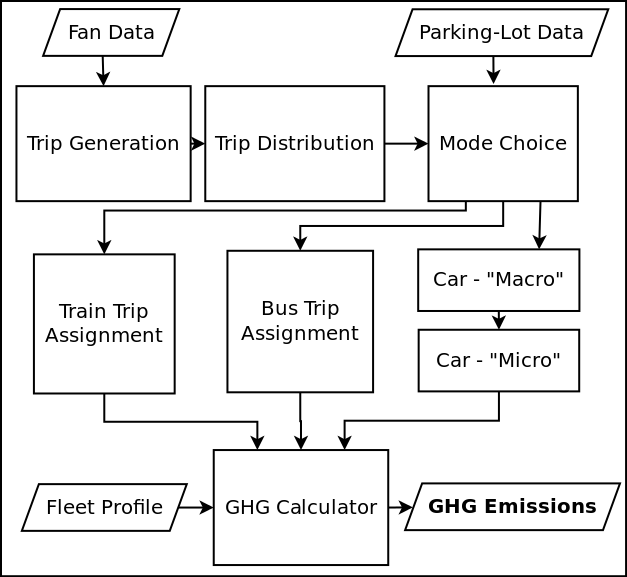
\includegraphics[height=8cm]{fullsystem1.png}
  \caption{System block diagram of our phase 1 model}
  \label{mainsystem1}
\end{figure}

\begin{description}[style=nextline]
    \item[Trip Generation] We will need to gather data on the
  geographic distribution of the fans that attend the games. We hope
  to obtain a good amount of data from the Eagles to aid in this
  section. Absent that data, we will have to resort to theoretical
  models commonly used in the industry, such as the Gravity Model. We
  will also be gathering data on timing of the trips, either through
  direct observation, or ideally from already existing records.
    \item[Trip Distribution] This step in the modeling is
  straightforward, since we know that fans are traveling to and from
  the stadium (or a nearby parking lot).
    \item[Mode Choice] This phase involves matching each trip in the
  database to a mode of travel (i.e. Car vs. SEPTA vs. Bus). We plan
  on using parking-lot data to estimate car use, and, if possible, get
  station-level information directly from SEPTA. A variety of
  theoretical models exist to help validate the gathered data.
    \item[Trip Assignment] Is the selection of the specific lines,
  streets, highways, and stations that each trip will follow. At this
  stage, we will break the model into subsystems for each of the
  possible means of transportation.
    \begin{description}[style=nextline]
        \item[Trains] A great deal of information is available on the
      website regarding lines and schedules that we have used to build
      a software representation of the network. With some
      well-established linear optimization algorithms, we will be able
      to model the exact path taken for every trip assigned to SEPTA
      trains. A preliminary step is to populate the station model, as
      shown in figure \ref{septa-db}. Then, we will use established
      algorithms to run the model based on this database, as shown in
      figure \ref{septa}
        \item[Buses] Schedules and stops are also available at
      www.septa.org. We will merge this database with the
      information available on Google Maps to obtain location data.
      There are also well-established algorithms we can use to model
      the paths of every trip.
        \item[Cars] Our car model will be split in two: \label{cars}
      \begin{itemize}
          \item At a "micro" level, we will model the road network in
        and around the stadium parking lot based on existing databases
        complemented with hand-input data that we extract from maps
        and planning documents. This portion will be used to model the
        exiting cars, since we believe the congestion at the end of a
        game results in substantial GHG emissions.
          \item At a "macro" level, we will use the same TAZs as in
        the trip generation phase, and calculate a sample path to the
        stadium based on highways and main roads.  We will have to
        encode the network of such roads and use our own algorithms.
        Alternatively, depending on the resulting number of TAZs, and
        subject to special authorization, we could use the Google Maps
        API to programmatically retrieve routing information.
      \end{itemize}
    \end{description}
      \item[GHG Calculator] This subsystem will be a memoryless
    function mapping a trip to an estimated emissions value. Our
    preliminary assumption is that trips taken on public transit
    contribute no additional GHG, since we are taking the bus and
    train schedules as given. For cars, there are a multitude of
    published methods for estimating emissions. We will have to
    estimate a fleet profile (average age and size) to use one of
    these models. We expect that it will be a function of total
    highway distance/time, local street distance/time, and idling
    time. When properly built, the output from this subsystem will be
    our first main deliverable.
\end{description}

\begin{figure}[htp]
  \centering
  \begin{subfigure}{.504\textwidth}
    \centering
    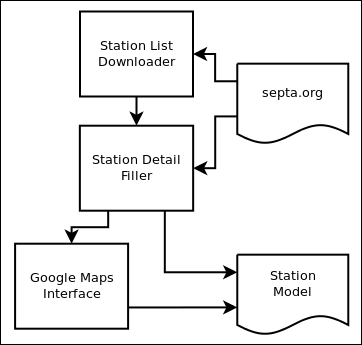
\includegraphics[width=\textwidth]{septa-db.png}
    \caption{Populating the station database}
    \label{septa-db}
  \end{subfigure}
    \begin{subfigure}{.394\textwidth}
    \centering
    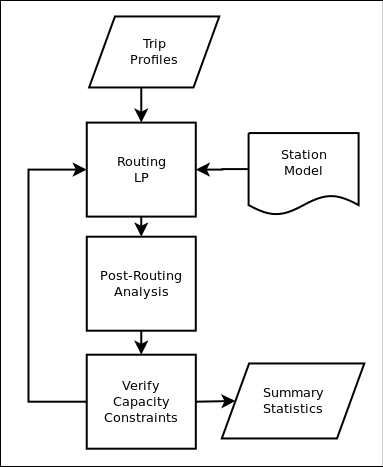
\includegraphics[width=\textwidth]{septa.png}
    \caption{Operation of the train subsystem}
    \label{septa}
  \end{subfigure}
  \caption{Components of the SEPTA Train Model}
% septa.png 383 w x 467 h
% septa-db.png 362 w x 345 h
% w1 * 467 / 383 = w2 * 345 / 362
% w2 = w1 * (467 * 362) / (383 * 345) = w1 * 1.2794
% w1 + w2 = .9\textwidth
% w1 = .9\textwidth / ( 2.27924)
%    = .394\textwidth
% w2 = .504\textwidth
\end{figure}

For the second phase of the project, as mentioned above, we will seek
to leverage as much of the modeling work from phase one as
possible. The goal for this phase will be to focus on converting the
existing model into a usable simulator. A key objective will be
incorporating a variety of inter-system feedback mechanisms that will
allow for a more accurate model.  The degree of detail in these
feedbacks mechanism will be constrained by the computational
complexity of including them (see Table \ref{specs} for computational
requirements) and by the design constraints of our subsystems (see
Section \ref{requirements}) Since there may be limited opportunities
to validate our model (until the next season begins), a key
performance metric will be the consistency of results, which in
technical terms, means that the system should reject small
disturbances in the inputs.  Conceptually, changing the base fare for
SEPTA or increasing the cost of parking by small amounts should not
result in wildly different behavior. This sensitivity will be a key
measure we will use in determining the right level of complexity to
build into the model.

Some examples of feedback mechanisms we are considering at this stage
are:

\begin{description}[style=nextline]
    \item[Congestion] If a fan spends 45 minutes stuck in the parking
  lot unable to move, we expect that fan to be more likely to take the
  train for the next game. A more detailed discussion of the fan model
  lies below.
    \item[Scheduling] If SEPTA notices trains traveling fuller on game
  days, they may choose to alter schedules in the future.
    \item[Uncertainty Effects] As fans try different modes of
  transportation, they may refine their predictions of travel times
  and convenience.
    \item[Fleet Composition] We suspect the fans that are most likely
  to start using public transit may have cars with above-average fuel
  efficiency, whereas the fans that take their trucks to tail-gate
  parties will likely continue to use their less-efficient cars.
  These effects would alter the fleet profile and hence average
  emissions calculations.
\end{description}

Regardless of what feedback loops we ultimately incorporate, we will
have to build a model of the fans' utilities, to capture the effects
of the various incentive schemes on trip generation profiles. At this
stage we expect we will be using an agent-based technique for this
subsystem, which will have as inputs the TAZs and some demographic
data. Cooperation from the Eagles will be important in fine-tuning
this part of the model.

The expanded model can be seen in the block diagram in figure
\ref{mainsystem2}. We have included the incentive structure as an
input in the diagram. We expect to make a GUI for this input to the
model, which will have a variety of options. For now, we have left
these unspecified as we will have to discuss with the Eagles what
their interests are. The other block added is the preference model,
which will be an agent- or automata-based model about fan preferences,
i.e. how they value travel time, convenience, comfort, and other
parameters that differ between the different modes of transportation.

\begin{figure}[htp]
  \centering
  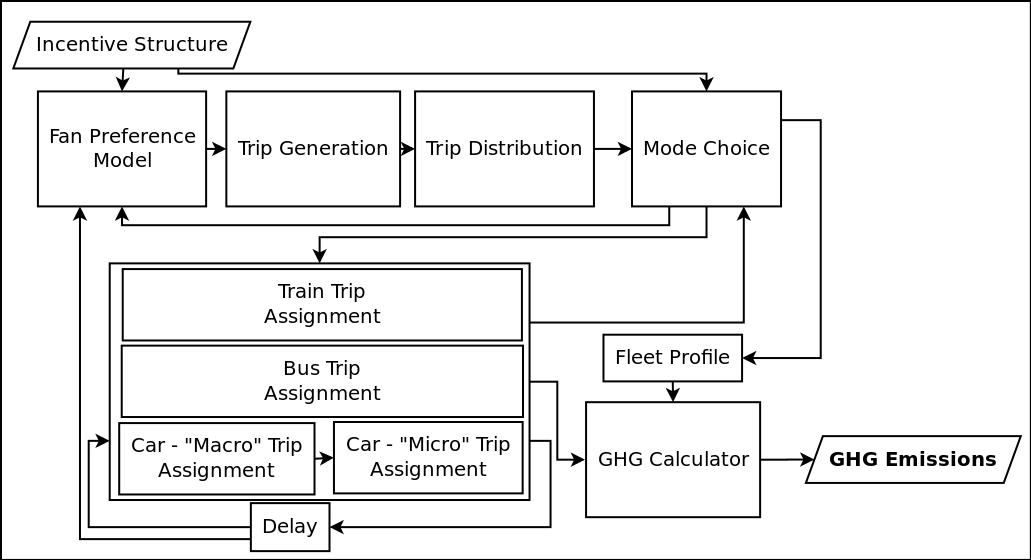
\includegraphics[height=8cm]{fullsystem2.png}
  \caption{Full system incorporating feedback}
  \label{mainsystem2}
\end{figure}

\subsection{System Specification}
Our end system must have a GUI that can be used by Eagles management
to input proposed incentives and that will output the projected change
in GHG. The input must be intuitive and friendly enough that it does
not require a manual for a user of average computer literacy to learn
to use it in 10 minutes or less. Additionally, once a user is familiar
with the interface, varying parameters on a proposed incentive program
should not require more than 2 minutes of the user's time.

The back-end must be flexible and have a documented API so that a
software developer may write extensions to the model (e.g. different
incentive types) or refine sub modules (e.g. a more efficient traffic
assignment subsystem) without having to modify the other components of
the software. Additionally, the model must be fast enough so that
initial estimates of GHG emissions under certain incentive schemes may
be computed within 5 minutes. In addition, detailed logs and reports
(e.g. emissions over time graphs) should be accessible to a more
knowledgeable user through the same GUI.

The program must handle improper input robustly and must be able to
deal with exceptions and errors gracefully. Specifically, a user of
average computer literacy should be able to understand error messages,
and, in a worst-case scenario, should be able to simply reset the
application to restore functionality.

The subsystem specifications are laid out in table \ref{specs}
\begin{table}[htp]
  \newlength\midcolumnwidth
  \midcolumnwidth=.74\textwidth plus 10\tabcolsep minus 10\tabcolsep
  \centering
  \caption{Specifications table}
  \label{specs}
  \begin{tabular}{%
    >{\raggedright}p{.11\textwidth}%
    p{\midcolumnwidth}%
    >{\raggedright\arraybackslash}p{.15\textwidth}}
  \firsthline
  \bfseries Module & \bfseries Qualitative Requirements & \bfseries
  Quantitative Performance Requirements \\ \hline
  Trip Generation & Interface with a database of TAZs and (if
  possible) a database of sanitized user data in strict XML format.
  Output a list of trips specifying the origin and time of each one. &
  $5\,s$ per $50,000$ trips \\
  Trip Distribution & Pass through the list from the trip generation
  module. & N/A \\
  Mode Choice & Read in sanitized parking-lot data in SQL,
  station-level usage information, and TAZ demographic profiles.
  Assign a mode choice to each entry in the the list from the trip
  distribution module.
  Output a vector of the different trips in each category and
  summary statistics for each mode (e.g. utilization percentage). &
  $10\, s$ per $50,000$ trips \\
  Trains & Read in a line and schedule XML database
  and accept an input of trip origin and time pairs. Calculate the
  most direct path to the stadium for each trip , subject to capacity
  constraints. Output summary statistics and trip list. & $1\,$min
  per 50,000 trips \\
  Buses & As above, with its own (larger) database. The trip profiles
  must not specify stop-by-stop, but rather total distance, to
  within 5\% error. & $1\,$min per 50,000 trips \\
  Cars & (See below) & $1\,$min per 50,000 trips total \\
  Cars - Micro & Accept the list of trips and read in a database of
  the road network in and around the stadium. Compute total distance
  and idling time per car to reach the highways/main roads. & \\
  Cars - Macro & Accept the same list of trips as above and compute
  total highway and secondary road times across all trips. Optionally
  interface with the Google Maps API. & \\
  GHG Calculator & Process the outputs from the trip assignment
  modules and compute an overall level of GHG emissions. & $10\,s$
  per 50,000 trips \\
  \lasthline
  \end{tabular}
\end{table}
\subsection{Hardware and Software Requirements}
\subsubsection{Hardware Requirements and Design Approach}
The hardware requirements for this project will feature towards the
tail end of the project.  The end-user (be it the Eagles/Phillies or
the policemen directing traffic), will be receiving a finished piece of
software from us, which would require specialized hardware to deal
with it.

In order to make the software/algorithm we create generalizable, we
will be utilizing a popular hardware choice of either a personal
computer or a portable device (iOS/Android). The choice will be made
upon further discussion with the Eagles and at this time we are unable
to provide reasons for a technical hardware choice.

\subsubsection{ Software Requirements and Design Approach}
The software we create will be created primarily in Matlab and
Python. The requirements we have from our software will be as follows:
\label{requirements}
\begin{description}[style=nextline]
    \item[Modularity] We should we able to switch out one
  implementation of the train model, for instance, and replace it
  seamlessly with another, more efficient implementation.
    \item[Scalability] It should be able to handle a large number of
  inputs and not break under scale. It will have to deal with tens of
  thousands of fans inhabiting the model.
    \item[User-Friendliness] We want the final output, or GUI, to be
  extremely user-friendly and it should be operational without a
  manual.
\end{description}

We expect to use commonly available hardware. In summary, we will be
looking to create a model that takes in data about demand generation
and incentives and uses that to determine the modal usage of
transportation to Eagles games.  Finally, we will be using the model
to determine the amount of time cars idle and based on expected CO2
emission rates, we will be determining the impact of the incentives
inputted into the model. We will also be developing a module to
incorporate feedback, allowing for ``state'' in our model (i.e. prior
experiences impact future choices).


\addtocounter{subsection}{1} %\subsection{Test and Demonstration}
%\subsubsection{Test}
%\subsubsection{Demonstration}

\subsection{Schedule}
The schedule consists of the different tasks that we estimate we will
need to accomplish in order to have a successful project. The tasks
can be broken into

\begin{itemize}
  \item Planning and design
  \item Creating the required subsystems
  \item Integrating the subsystems into one system
  \item Implementation.
\end{itemize}

Each task is assigned to only one individual although others may also
be working on the tasks, but the assigned individual is accountable to
get it done correctly and on time. Based on the Gantt chart and
schedule it is clear that we aim to work consistently over the course
of the year to meet the milestones (course requirements) and also aim
to get some work done over winter break so that we don’t fall behind
schedule.

We are currently ahead of schedule in some tasks, and behind schedule
in other tasks. This is similar to our situation when we submitted the
first project report because we are facing similar obstacles in
obtaining required information to progress in certain areas. However,
this is not as much of a concern to us as being completely behind
schedule because we can alter resource allocation to reconcile the
variance and bring the project back on schedule.

The two areas where we are behind schedule are:

\begin{enumerate}[label=(\emph{\alph*})]
  \item Working with the Philles/Eagles
  \item Working with the Philadelphia Police Department.
\end{enumerate}

This can be attributed to the major constraint mentioned in the
introduction. Dr. Huemmler has been trying to get us in touch with
them, but so far they have not been very responsive.

On November 16th, 2012, Dr. Huemmler sent letters on SEAS letterhead
paper to the following five individuals in these organizations:
\begin{description}[style=nextline]
    \item[Mike DiMuzio]
  Director of Operations/Facilities, Philadelphia Phillies
    \item[Julie Hershey]
  Community Relations, Philadelphia Eagles
    \item[Zach Hill]
  Senior Director of Communications, Philadelphia Flyers
    \item[Michael Preston]
  Director of Public Relations, Philadlephia 76ers
    \item[Lt. John Hewitt]
  PSA Lieutenant
\end{description}

Dr. Huemmler assures us that we will have meetings set up for the
middle of January, when we return from winter break. We have formed a
contingency plan, and updated the schedule so that we can allocate
more time to this to bring us back on schedule once we have
established contact. We plan to devote more resources to the subtasks
that rely on the meetings in order to bring the project back on
schedule.

Although the delay in contract with the Eagles and Philadelphia PD
lead us to fall behind in certain areas, we were able to reallocate
the time and resources that should have been used there, to other
tasks. These tasks include the SEPTA subsystem and GHG emissions
subsystem. Although we had originally planned to start these later in
this semester and next semester (respectively), we were able to start
and make progress on both of these subsytems during this semester.

Another factor that helped us get ahead of schedule in these areas was
the fact that we over-estimated the time to complete specific
tasks. The specific tasks that we over-estimated were the research to
find the necessary data for the GHG emissions subsystem and the
programming aspect of the SEPTA subsystem.

Overall, at the end of the first semester we have made significant
progress, which is discussed in more detail in the Results section. We
have defined our problem and scope, designed our systems approach and
began building two of the subsystems. We also plan to have some work
done over winter break, and consolidate our efforts at the beginning
of next semester and revise our schedule accordingly.

\section{Preliminary Results}
As discussed in the schedule discussion in section 3.5, we have made
significant progress on our project that will be critical to
supporting our efforts in Phase 2. We have had four main outcomes from
Phase 1 that we hope to carry forward.

\subsection{Project scope and determination of target user}

Our project started off with the aim of reducing CO2 emissions from
cars idling in parking lots after sports games. Over the course of
Phase 1, we have broadened our scope to develop a system to reduce GHG
emissions as a byproduct of fans travelling to and from sports
games. This broad aim will be carried forward to Phase 2 to drive us
to find innovative solutions to problems that we face by keeping the
overall goal in mind.

Through the semester, we have also determined three possible target
users for the finished product from our project:

\begin{descenum}
    \item[Philadelphia Sports Teams] (Eagles/Phillies/Flyers) We could
develop an interface that would allow the management of these teams to
determine the impact of various incentives towards reducing GHG
emissions.

  \item[Philadelphia Police Department] We could develop a mock-up of
an application that would help streamline traffic direction for fans
leaving stadiums

  \item[Sports Fans] We could develop a web interface/mock-up that would
allow users to understand the GHG emission impact of their travels and
alternatives to reduce this impact.
\end{descenum}

Our work in Phase 2 will involve determining which target user would
be the best choice to focus on given the availability of data and
involvement of the sports teams (as talked about before in the
report).

\subsection{Overall systems approach}
As discussed in section 3.1, we
have developed an overall systems approach to the project that we will
be using to guide our progress next semester. The system block diagram
will be used to understand how each module fits into the overall
system and will help prioritize among competing choices for time
allocation.

\subsection{SEPTA Subsystem}
Through Phase 1, we have developed a comprehensive database of all
SEPTA rail, trolley and transit stations and the lines that operate
across these stations. This data is stored in a well-typed XML based
on a DOM that ensures that all required fields are present for each
station. This database will be used to support further development of
the train model in calculating the emissions from the train system as
well as travel time alternatives when suggesting substitution of car
travel with train travel.

\subsection{GHG Emissions Subsystem}
Through Phase 1, we
have developed a comprehensive plan to create the GHG emissions
subsystem. The discussion above already detailed the creation and
design of the system, including the input, transfer function and
output for each of the five iterations. This plan will be used in
Phase 2 to program the subsystem and create a working model of the GHG
emissions subsystem.

\addtocounter{section}{1} % \section{Lessons Learned}

\section{Equipment/Fabrication/Software Needs}
We do not have any need for specialized equipment or software. The
software we will be using is either publicly available, or available
at Penn. We expect that our production version of the model will not
depend on commercial tools.

\addtocounter{section}{1} % \section{Conclusions and Recommendations}

\section{Nomenclature}
{\centering
\midcolumnwidth=.8\textwidth plus 10\tabcolsep minus 10\tabcolsep
\begin{tabular}{%
    >{\raggedright\bfseries}p{.1\textwidth}%
    p{\midcolumnwidth}}
  API & Application programming interface. An official, documented way
  for a program to access a database or another program, such as that
  of Google Maps. \\
  DOM & Document Object Model. A file format that is very easy to
  parse and yet human-readable. \\
  EPP & Emissions per passenger. \\
  EPM & Emissions per mile. \\
  GHG & Greenhouse gases. We mostly mean Carbon Dioxide, but we use
  the term GHG since emissions are highly correlated across types in
  this application. \\
  HBO & Home-based other. A category of trips in the
  standard  model. Contrast with HBS, HBW, NHO, and NHW. \\
  HBS & Home-based shop. A category of trips in the standard
  model. Refers to trips from the home to go shopping. Contrast with
  HBO, HBW, NHO, and NHW. \\
  HBW & Home-based work. A category of trips in the standard
  model. Refers to trips from the home to go to work. Contrast with
  HBO, HBS, NHO, and NHW. \\
  MAG & Maricopa Association of Governments. It is in charge of
  transportation planning for Phoenix and it surroundings. \\
  NHO & Non-home-based other. A category of trips in the standard
  model. Contrast with  HBO, HBS, HBW, and NHW. \\
  NHW & Non-home-based work. A category of trips in the standard
  model. Refers to trips not from the home to go to work. Contrast
  with HBO, HBS, HBW, and NHO. \\
  SEPTA & Southeast Pennsylvania Transit Authority. Manages the
  commuter rail, the subway, trolley, and bus systems in and around
  Philadelphia \\
  SQL & A type of database that is commonly used. \\
  TAZ & Traffic analysis zone. Used in modeling the UTMS. It involves
  dividing a geographical area into units that have sufficiently
  similar transit and demographics to treat as one for the purposes of
  the model. \\
  UTMS & Urban Transportation Modeling System. A commonly used
  framework to model traffic demand and flows. \\
  XML & Extensible markup language. A structured file format that is
  human-readable and easily parseable and customizable. \\
\end{tabular}
}

\makereferences

\makebibliography


\section{Financial Information}
We expect our project to incur minimal cost. At this time, the only
foreseeable expenses are the cost of transportation to the
stadium. Depending on how we refine the user needs after our meeting
with the Eagles, we may have to purchase a mobile device on which to
prototype our model interface.

%\section{Ethical Issues}

\appendix

\section{A Documented Module of Code}
\fontsize{10}{12}\selectfont
\begin{verbatim}
#! /usr/bin/env/python3

"""
stations.py reads in an xml file containing a list
of station elements with name and url subelements.
It fetches those urls and tries to extract the lines
serving those stations from the websites. It updates
the xml and saves the updated list into a (potentially)
new file.

usage: $ python stations.py xml-file-name [output-name]

"""

import xml.etree.cElementTree as ET
import urllib.request
import re
from urllib.error import HTTPError


class Station:

    LINES_RE = re.compile("<p>This station is served by:<br ?/?>"
                          "(.+?)</p>", re.DOTALL)
    BREAK_RE = re.compile("<br ?/?>")
    PARKING_RE = re.compile('<table[^>]*>\s*<tr>\s*<td[^>]*>'
                            '<h2 class="normal">Parking</h2>'
                            '.*</table>', re.DOTALL)

    def __init__(self, element):
        self.element = element
        assert (self.element.find('url') is not None)
        self._html = ''
        self._lines = []
        self._parking = []

    @property
    def url(self):
        return self.element.find('url').text

    @property
    def html(self):
        if not self._html:
            self.update_html(self.url)
        return self._html

    def update_html(self, url):
        # UTF-8 encoded checked by hand on a couple of urls
        try:
            self._html = urllib.request.urlopen(url).read().decode('utf8')
        except HTTPError as e:
            self._html = "HTTP Error #" + str(e.code)

    @property
    def lines(self):
        if not self._lines:
            self.update_lines()
        return self._lines

    def update_lines(self):
        section = self.LINES_RE.search(self.html)
        try:
            section = section.group(1)
        except AttributeError:  # No match found
            self._lines = ["REGEX ERROR"]
            return
        section = section.strip()
        section = self.BREAK_RE.sub("\n", section)
        # subbing <br>s may result in double newlines,
        # and hence blank "entries"
        # That's why composition below is filtered
        self._lines = [s.strip() for s in section.splitlines()
                                                  if s.strip()]

    def set_lines(self):
        lines = self.element.find('lines')
        if lines is None:
            lines = ET.SubElement(self.element, 'lines')
        for line in self.lines:
            el = ET.SubElement(lines, 'line')
            el.text = line

    @property
    def parking(self):
        if not self._parking:
            self.update_parking()
        return self._parking

    def update_parking(self):
        section = self.PARKING_RE.search(self.html)
        try:
            section = section.group(0)
        except AttributeError:  # No match found
            self._parking = [("REGEX ERROR", 0, 0)]
            print("Regex error at " + self.url)
            return
        section = lowercase_tags(section).replace('&nbsp;', '')
        try:
            table = ET.fromstring(section)
        except ET.ParseError:
            try:
                # The first row does not appear to be closed properly
                # i.e., the terminal "</tr>" appears as "<tr>" instead
                section = section.replace("<tr>", "</tr>", 2)
                section = section.replace("</tr>", "<tr>", 1)
                table = ET.fromstring(section)
            except ET.ParseError as e:
                self._parking = [("MALFORMED HTML", 0, 0)]
                print("Malformed HTML at " + self.url)
                print(section)
                print(e)
                return
        rows = list(table)[1:]  # :FIXME:
        self._parking = []
        for row in rows:
            if len(row) == 1:
                # There is no parking. HTML should look like
                # <tr><td colspan="4">There is no parking available at this
                # station.</td></tr> with some whitespace thrown in.
                assert (row.find('td').text ==
                        "There is no parking available at this station.")
                self._parking = [('N/A', 0, 0)]
            else:
                assert len(row) == 4
                # Entries are: SEPTA, Spaces, Availability, Price
                entries = row.findall('td')
                del entries[2]
                def get_text(e):
                    t = e.text
                    try:
                        return t.strip()
                    except AttributeError:
                        return ''
                self._parking.append(tuple(get_text(td)
                                          for td in entries))

    def set_parking(self):
        pt = self.element.find('parking-lots')
        if pt is None:
            pt = ET.SubElement(self.element, 'parking-lots')
        for kind, size, price in self.parking:
            lot = ET.SubElement(pt, 'parking')
            t = ET.SubElement(lot, 'type')
            t.text = kind
            s = ET.SubElement(lot, 'size')
            s.text = size
            p = ET.SubElement(lot, 'price')
            p.text = price or "0"  # Parser ignores zeros, apparently


HTML_TAG = re.compile(r"</?([:_A-Za-z][:_A-Za-z\-]*) ?[^>]*>")
def lowercase_tags(html):
    """Converts all tag names in a block of html to lowercase."""
    def lowerize(match):
        full = match.group(0)
        name = match.group(1)
        return full.replace(name, name.lower())
    return HTML_TAG.sub(lowerize, html)


if __name__ == "__main__":
    import sys
    if len(sys.argv) > 3:
        print(__doc__)
        sys.exit(1)
    try:
        xmlfilename = sys.argv[1]
    except IndexError:
        print(__doc__)
        sys.exit(1)
    try:
        outname = sys.argv[2]
    except IndexError:
        outname = xmlfilename

    tree = ET.parse(xmlfilename)
    stations = [Station(e) for e in tree.iter(tag='station')]
    for station in stations:
        station.set_lines()
        station.set_parking()
    tree.write(outname)

\end{verbatim}

\end{document}

%  LocalWords:  DOM EPP EPM GHG Huemmler Vukan Vuchic ITE
